\section{Материалы предварительного проектирования системы}
\subsection{Функциональная схема обработки данных}

\begin{figure}[!htb]
    \centering
    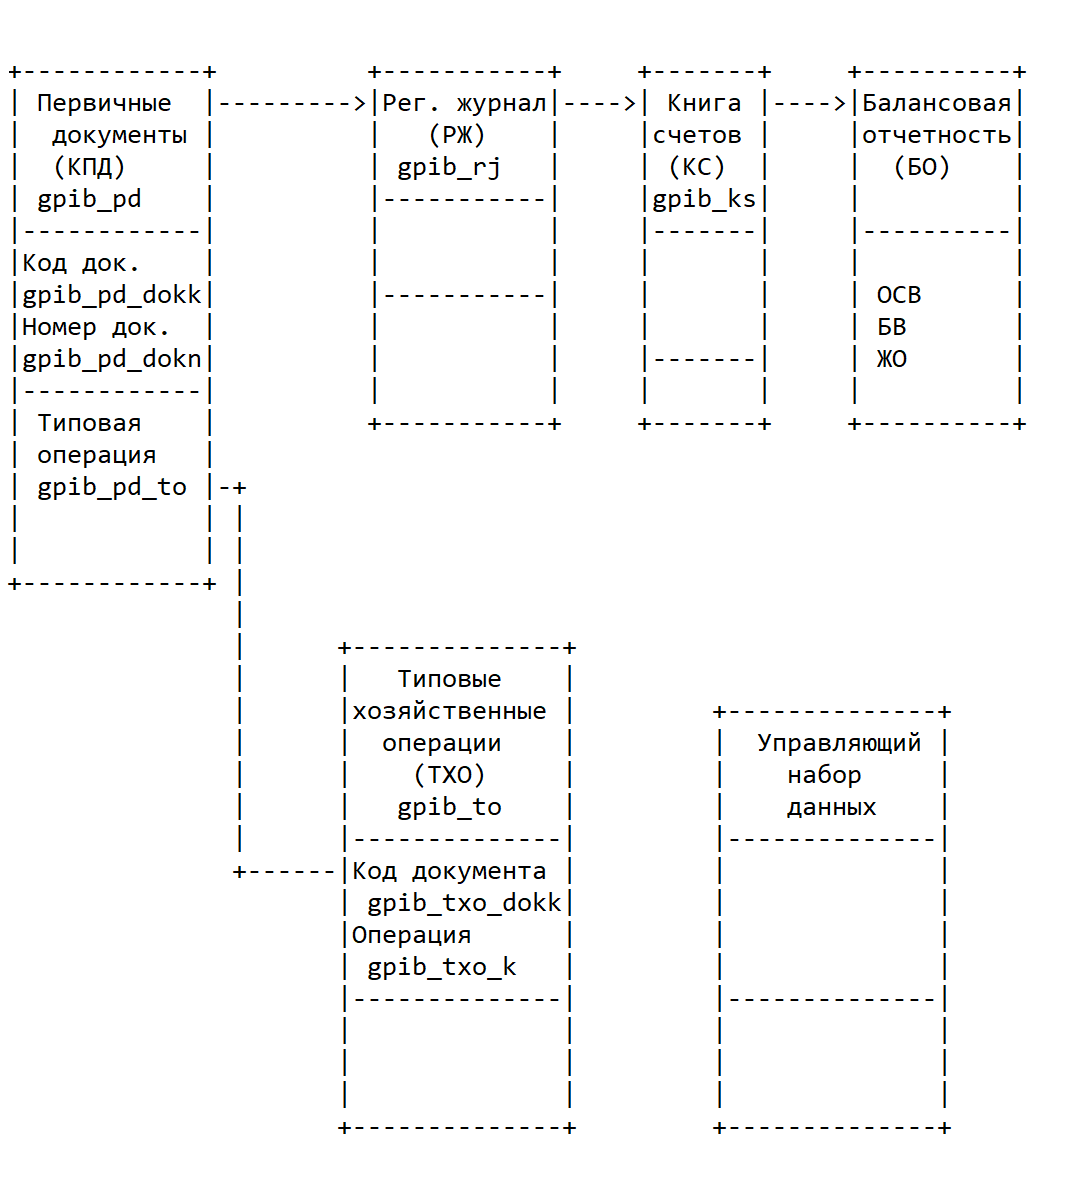
\includegraphics[width=18cm]
        {_assets/gpib_part2.png}
    \caption{Функциональная схема обработки данных}
\end{figure}

\newpage

\subsection{Описание картотек}

Картотеки:

\begin{itemize}
    \item Первичные документы \gpiFIO\/b\_pd;
    \item Регистрационный журнал (РЖ) \gpiFIO\/b\_rj;
    \item Книга счетов(КС) \gpiFIO\/b\_ks;
    \item Типовые хозяйственные операции (ТХО) \gpiFIO\/b\_to.
\end{itemize}

\begin{table}[!htb]
    \centering
    \scriptsize
    \caption{Первичные документы \gpiFIO\/b\_pd}
    \begin{tabular}{|p{7cm}|p{7cm}|c|}

\hline
\multicolumn{1}{|c}{\textbf{Реквизит}}
&\multicolumn{1}{|c}{\textbf{Обозначение}}  
&\multicolumn{1}{|p{1.6cm}|}{\textbf{Тип и значность}} 
\\ \hline

поле связи =0               &\gpiFIO\/b\_pd\_0            &n1                         \\ \hline
код документа < --- opd     &\gpiFIO\/b\_pd\_dokk         &c3                         \\ \hline
номер документа             &\gpiFIO\/b\_pd\_dokn         &n5                         \\ \hline
дата документа              &\gpiFIO\/b\_pd\_dokd         &d8                         \\ \hline
типовая операция < --- txo  &\gpiFIO\/b\_pd\_to           &c10                        \\ \hline
дебет *txo                  &\gpiFIO\/b\_pd\_db           &n2                         \\ \hline
дебет наименование *txo     &\gpiFIO\/b\_pd\_dbn          &c10                        \\ \hline
кредит *txo                 &\gpiFIO\/b\_pd\_kr           &n2                         \\ \hline
кредит наименование *txo    &\gpiFIO\/b\_pd\_krn          &c10                        \\ \hline
сумма                       &\gpiFIO\/b\_pd\_rub          &n10                        \\ \hline

    \end{tabular}
\end{table}

\newpage

\begin{table}[!h]
    \centering
    \scriptsize
    \caption{Регистрационный журнал (РЖ) \gpiFIO\/b\_rj}
    \begin{tabular}{|p{7cm}|p{7cm}|c|} 

\hline
\multicolumn{1}{|c}{\textbf{Реквизит}}
&\multicolumn{1}{|c}{\textbf{Обозначение}}  
&\multicolumn{1}{|p{1.6cm}|}{\textbf{Тип и значность}} 
\\ \hline

поле связи =0                   &\gpiFIO\/b\_rj\_0            &n1                         \\ \hline
дата операции                   &\gpiFIO\/b\_rj\_data         &d8                         \\ \hline
код оправдательного документа   &\gpiFIO\/b\_rj\_dokk         &c3                         \\ \hline
номер документа                 &\gpiFIO\/b\_rj\_dokn         &n10                        \\ \hline
дата документа                  &\gpiFIO\/b\_rj\_dokd         &d8                         \\ \hline
содержание операции             &\gpiFIO\/b\_rj\_to           &c10                        \\ \hline
дебет, счет                     &\gpiFIO\/b\_rj\_db           &n2                         \\ \hline
дебет, наименование             &\gpiFIO\/b\_rj\_dbn          &c10                        \\ \hline
кредит, счет                    &\gpiFIO\/b\_rj\_kr           &n2                         \\ \hline
кредит наименование             &\gpiFIO\/b\_rj\_krn          &c10                        \\ \hline
сумма                           &\gpiFIO\/b\_rj\_rub          &n10                        \\ \hline

    \end{tabular}
\end{table}

\begin{table}[!htb]
    \centering
    \scriptsize
    \caption{Книга счетов(КС) \gpiFIO\/b\_ks}
    \begin{tabular}{|p{7cm}|p{7cm}|c|} 

\hline
\multicolumn{1}{|c}{\textbf{Реквизит}}
&\multicolumn{1}{|c}{\textbf{Обозначение}}  
&\multicolumn{1}{|p{1.6cm}|}{\textbf{Тип и значность}} 
\\ \hline

поле связи =0                   &\gpiFIO\/b\_ks\_0            &n1                         \\ \hline
дата операции                   &\gpiFIO\/b\_ks\_data         &d8                         \\ \hline
код оправдательного документа   &\gpiFIO\/b\_ks\_dokk         &c3                         \\ \hline
номер документа                 &\gpiFIO\/b\_ks\_dokn         &n10                        \\ \hline
дата документа                  &\gpiFIO\/b\_ks\_dokd         &d8                         \\ \hline
операции                        &\gpiFIO\/b\_ks\_to           &c10                        \\ \hline
счет                            &\gpiFIO\/b\_ks\_s            &n2                         \\ \hline
счёт наименование               &\gpiFIO\/b\_ks\_sn           &c10                        \\ \hline
кор. счёт                       &\gpiFIO\/b\_ks\_ks           &n2                         \\ \hline
кор. счет наименование          &\gpiFIO\/b\_ks\_ksn          &c10                        \\ \hline
сумма дб                        &\gpiFIO\/b\_ks\_rubdb        &n10                        \\ \hline
сумма кр                        &\gpiFIO\/b\_ks\_rubkr        &n10                        \\ \hline

    \end{tabular}
\end{table}

\begin{table}[!htb]
    \centering
    \scriptsize
    \caption{Типовые хозяйственные операции(ТХО) \gpiFIO\/b\_txo}
    \begin{tabular}{|p{7cm}|p{7cm}|c|}

\hline
\multicolumn{1}{|c}{\textbf{Реквизит}}
&\multicolumn{1}{|c}{\textbf{Обозначение}}  
&\multicolumn{1}{|p{1.6cm}|}{\textbf{Тип и значность}} 
\\ \hline

поле связи =0                   &gpi\_to\_0             &n1                         \\ \hline
код документа < --- opd         &gpi\_to\_dokk          &c3                         \\ \hline
код типовой операции            &gpi\_to\_k             &c10                        \\ \hline
дебет, счёт < --- ps\_1         &gpi\_to\_db            &n2                         \\ \hline
дебет, наименование * ps\_1     &gpi\_to\_dbn           &c10                        \\ \hline
кредит < --- ps\_2              &gpi\_to\_kr            &n2                         \\ \hline
кредит, наименование * ps\_2    &gpi\_to\_krn           &c10                        \\ \hline

    \end{tabular}
\end{table}

\newpage

\subsection{Описание работ}

\begin{table}[!htb]
    \centering
    \scriptsize
    \caption{Описание работ}
    \begin{tabular}{|p{6cm}|p{11cm}|} 

% = = = = = = = = = =

\hline
\multicolumn{1}{|c}{\textbf{Группа работ}}
&\multicolumn{1}{|c|}{\textbf{Работы}}
\\ \hline

% = = = = = = = = = =

Формирование и разноска первичных \par
документов \par
\hspace{0pt} \par
\textbf{\gpiFIO\/b\_Документы}
&
- \gpiFIO\/b\_Ввод текущей даты \par
- \gpiFIO\/b\_Ввод и разноска первичных документов(ПД)
\\ \hline

% = = = = = = = = = =

Работа с регистрационным журналом \par
\hspace{0pt} \par
\textbf{\gpiFIO\/b\_РЖ}
&
- \gpiFIO\/b\_Просмотр РЖ \par
- \gpiFIO\/b\_Формирование КС и РЖ \par
- \gpiFIO\/b\_Просмотр КС \par
- \gpiFIO\/b\_Сформировать КС на печать \par
- \gpiFIO\/b\_Просмотр КС для печати
\\ \hline

% = = = = = = = = = =

Формирование балансовой отчетности \par
\hspace{0pt} \par
\textbf{\gpiFIO\/b\_БО}
&
- \gpiFIO\/b\_Опеделение отчетных форм \par
- \gpiFIO\/b\_сформировать КС на печать \par
- \gpiFIO\/b\_ Просмотр КС для печати \par
- \gpiFIO\/b\_Сформировать ОСВ \par
- \gpiFIO\/b\_Просмотр ОСВ \par
- \gpiFIO\/b\_Сформировать Ж-О \par
- \gpiFIO\/b\_ Просмотр Ж-О \par
- \gpiFIO\/b\_Сформировать БВ \par
- \gpiFIO\/b\_ Просмотр БВ
\\ \hline

% = = = = = = = = = =

Сопровождение картотек-справочников \par
\hspace{0pt} \par
\textbf{\gpiFIO\/b\_Картотеки}
&
- \gpiFIO\/b\_Определение первичных документов \par
- \gpiFIO\/b\_Типовые хозяйственные операции(ТХО) \par
- \gpiFIO\/b\_Настройка АРМа
\\ \hline

% = = = = = = = = = =

Ведение архивов \par
\hspace{0pt} \par
\textbf{\gpiFIO\/b\_Архивы}
&
- \gpiFIO\/b\_Копия АРМ \par
- \gpiFIO\/b\_Восстановление АРМ
\\ \hline

% = = = = = = = = = =

Выход из системы \par
\hspace{0pt} \par
\textbf{\gpiFIO\/b\_Выход}
&
- \gpiFIO\/b\_Выход из системы
\\ \hline

% = = = = = = = = = =

    \end{tabular}
\end{table}

\newpage
